\begin{exercise}
      {ID-527580af7f290a075c04c661d88c5e534f343d3d}
      {Die Fliege und der Würfel}
  \ifproblem\problem\par
    Eine Fliege sitzt auf der Ecke $A$ eines Würfels und möchte zur Ecke $B$.
    Sie darf jeden möglichen Weg benutzen, nur durch das Innere des Würfels
    kann sie nicht. Sie möchte auf einer möglichst kurzen Strecke von $A$
    nach $B$ krabbeln. Wie sieht ihr Weg aus, und wie lang ist er?
    \begin{center}
      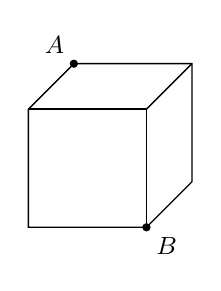
\begin{tikzpicture}[scale=1.5]
        \draw[line width=0.5pt] (0, 0, 1) -- (1, 0, 1) -- (1, 0, 0) -- (1, 1, 0) -- (0, 1, 0) -- (0, 1, 1) -- cycle;
        \draw[line width=0.5pt] (0, 1, 1) -- (1, 1, 1) -- (1, 0, 1);
        \draw[line width=0.5pt] (1, 1, 1) -- (1, 1, 0);
        \fill (0, 1) circle (1pt) node[above left] {{\small$A$}};
        \fill (0.615, -0.385) circle (1pt) node[below right] {{\small$B$}};
      \end{tikzpicture}
    \end{center}
  \fi
  \ifoutline\outline\par
    Stelle dir das Problem zweidimensional vor\ldots
  \fi
  %\ifoutcome\outcome\par
  %\fi
\end{exercise}
